\documentclass[conference]{IEEEtran}

\usepackage{graphicx} % For including images
\usepackage{amsmath} % For mathematical symbols and equations
\usepackage{hyperref} % For hyperlinks
\usepackage{caption}
\usepackage{amsfonts} % For math fonts and symbols
\usepackage{booktabs} % For better tables
\usepackage{listings} % For code listings
\usepackage{multirow} % For multi-row cells in tables
\usepackage{float} % For float image

\begin{document}
	
	\title{Data Management \\ Project of a Data Warehouse System for Analyzing Meteorite Landings by NASA}
	
	\author{
		\IEEEauthorblockN{Giuseppe Valente - Natalia Maria Mucha}
		\IEEEauthorblockA{
			Engineering in Computer Science \\
			Sapienza University of Rome \\
		}
	}
	\maketitle
	
	\begin{abstract}
			This project focuses on designing and developing a data warehouse (DWH) system to integrate and analyze meteorite landing data from NASA. The objective is to demonstrate the design and implementation of a data warehouse using a relational database (PostgreSQL), starting from the datasets.
	\end{abstract}
	
	\section{Introduction}
	
	This project aims to design and develop a DWH system specifically to integrate and analyze meteorite landing data using NASA's Meteorite Landings dataset. The first section focuses on both the design and development of the DWH, beginning with the Dimensional Fact Model (DFM), followed by the implementation of the Star Schema and the database itself. The second section is dedicated to the system architecture, detailing the components used, including the Extraction, Transformation, and Loading (ETL) processes, and how these tools are implemented. Docker containers are utilized to manage the DWH system, providing portability and simplicity. The final section contains the Git repository with the source code used for this project.
	
	\section{Data Warehouse}
	A DWH is a system used for reporting and data analysis. It serves as a central repository of integrated data from one or more sources (datasets or data sources). It stores both current and historical data in a single location, which is used for generating reports. This is beneficial for companies as it enables them to query and draw insights from their data, facilitating informed decision-making.

	The data stored in the DWH is uploaded from operational systems but first undergoes a process to ensure data quality before being used in DWH analysis (ETL process).

	The DWH employs a multidimensional model represented in \textbf{facts} that are subjects of analysis and represented as cubes, where:
	\begin{itemize}
		\item Each cell contains numerical \textbf{measures} (quantifying the fact from one perspective).
		\item Each axis represents a \textbf{dimension} of interest for analysis.
		\item Each dimension can be associated with a \textbf{hierarchy of dimensional attributes} used to aggregate data stored in the cubes.
	\end{itemize}

	To retrieve information from the DWH, four methodologies are used:
	\begin{itemize}
		\item Reports
		\item Dashboards
		\item Data mining
		\item OLAP
	\end{itemize}
	 
	\section{Requirements}
	\label{sec:requirements}
	We are interested in analyzing meteorite landings; for this reason, we use the following information:
	\begin{itemize}
		\item \textbf{Measure:} Meteorite mass in grams
		\item \textbf{Dimensions:} Time, Location, Meteorite Classification
	\end{itemize}
	\section{Dimensional Fact Model (DFM)}
	Starting from section\ref{sec:requirements} we designed the DFM model shown in Figure \ref{fig:Meteorite Landings System Architecture}. \\This figure illustrates the use of dimensional hierarchies for all dimensions, as well as optional dimension values.
	\begin{figure}[htpb]
		\centering
		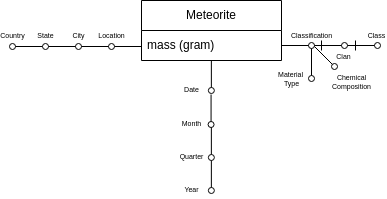
\includegraphics[width=\columnwidth]{images/dfm_schema.png}
		\caption{Meteorite Landings System Architecture}
		\label{fig:Meteorite Landings System Architecture}
	\end{figure}
	\section{Star Schema}
	A multidimensional structure can be represented using two distinct logical models:
	\begin{itemize}
		\item MOLAP (Multidimensional On-Line Analytical Processing)
		\item ROLAP (Relational On-Line Analytical Processing)
	\end{itemize}
	For our purpose we used the ROLAP model with the star schema.\\ Figure \ref{fig:Meteorite Landings Star Schema} describe the translation from the DFM to the Start Schema using the literature:
	\begin{figure}[htpb]
		\centering
		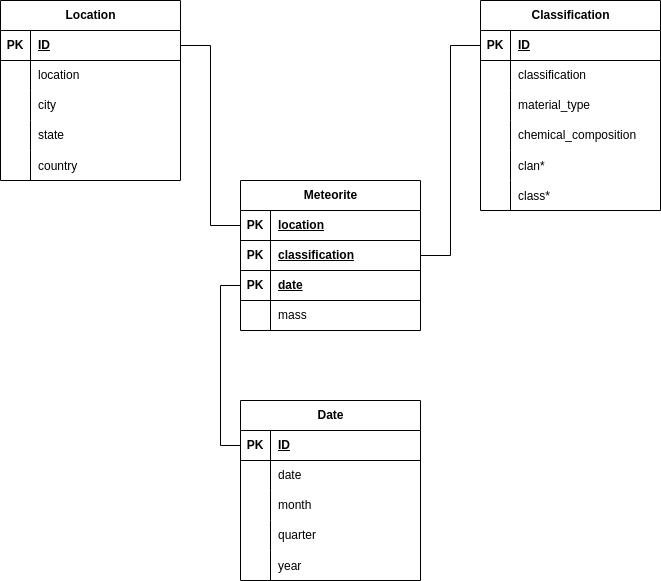
\includegraphics[width=\columnwidth]{images/star_schema.png}
		\caption{Meteorite Landings Star Schema}
		\label{fig:Meteorite Landings Star Schema}
	\end{figure}
	
	\section{System Architecture}
	The DWH architecture generally comprises the following components:
	\begin{itemize}
		\item \textbf{Datasets:} Collections of structured data organized to support reporting, analysis, and decision-making. These datasets are derived from various sources and are typically arranged to optimize querying and analysis.
		\item \textbf{ETL:} Stands for Extract, Transform, Load. It is a process used in data warehousing to move data from source systems to the data warehouse.
		\item \textbf{Primary DWH:} Refers to the central repository where an organization consolidates, stores, and manages its key business data for analysis and reporting. It is designed to support decision-making by providing a comprehensive view of data from various sources.
		\item \textbf{Data Mart:} A specialized subset of a DWH, designed to focus on a specific business area, department, or function. It is essentially a smaller, more focused version of a DWH that serves the needs of particular users or business units.
		\item \textbf{Reconciled Data (three-layer architecture only):} Refers to data that has been verified, adjusted, and aligned to ensure consistency, accuracy, and completeness across various sources or systems. The process of reconciling data involves comparing and aligning data from different sources to resolve discrepancies and ensure that the data is accurate and reliable.
	\end{itemize}
	
	The components are organized in either a two-layer or a three-layer architecture:	
	\subsection{Two-Layer Architecture (2LA)}
	The 2LA consists of two main components: the data sources and the DWH. In this architecture, data marts are considered part of the "presentation layer." This architecture is particularly useful for mid-sized to large organizations.
	\subsection{Three-Layer Architecture (3LA)}
	In this architecture, there is an additional layer: the reconciled data layer. This layer creates a common reference data model for the entire enterprise. It also clearly separates the issues of source data extraction and integration from those of DWH population. However, the reconciled data approach can lead to increased replication of operational source data, and the design process can be more complex.
			
	\subsection{Meteorite Landings - Architecture}
	For our purposes, we have opted to use the two-layer architecture (2LA) because we have a limited number of data sources, the ETL process is relatively simple, and it can be managed on the fly. However, in a real-world scenario, it would be advantageous to use a three-layer architecture (3LA). This architecture allows for the separation of Data Staging from Data Loading through the Reconciled Data Layer. Such separation facilitates the design of simpler and more efficient ETL tools, each focused on a specific task (e.g., \texttt{extract.py}, \texttt{transform.py}, \texttt{load.py}). Additionally, containerized technologies like Kubernetes or Docker can enable horizontal scaling of these tools, allowing the system to handle increased computational loads or growth in data sources more effectively.\\For simplicity, we use Docker to distribute the application in the most straightforward manner possible, but this does not imply that the application is scalable.\\As shown in Figure~\ref{fig:Meteorite Landings System Architecture}, our architecture includes the following components:
	\begin{itemize}
		\item \textbf{Datasets: (Meteorite Landings, Photon - Open Street Map)}
		\item \textbf{ETL: (meteorite\_landings\_etl)}
		\item \textbf{Primary DWH: PostgreSQL}  
	\end{itemize}
	\begin{figure}[htpb]
		\centering
		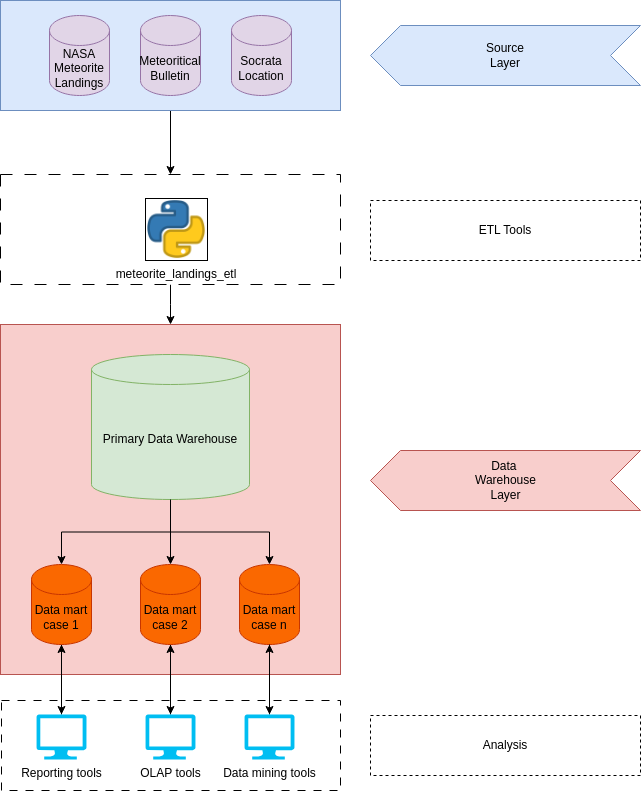
\includegraphics[width=\columnwidth]{images/system_architecture.png}
		\caption{Meteorite Landings System Architecture}
		\label{fig:Meteorite Landings System Architecture}
	\end{figure}
	
	\section{Source Layer}
	
	\subsection{Meteorite Landings Dataset}
	\label{subsec:meteorite landings data set}
	This comprehensive dataset from The Meteoritical Society contains information on all known meteorite landings. The Fusion Table was compiled by Javier de la Torre, and we have also provided an XLS file containing data on 34,513 meteorites. For additional details, visit \href{https://data.nasa.gov/Space-Science/Meteorite-Landings/gh4g-9sfh/about_data}{NASA's Open Data Portal}
		
	\subsection{Photon - Open Street Map}
	\label{subsec:open_street_map}
	The dataset is used to convert coordinate points from latitude and longitude to a human-readable format. For more information, see 
	\href{https://photon.komoot.io/}{Photon - Open Street Map}
				
	\section{ETL tools}
	The ETL process is carried out using \texttt{meteorite\_landings\_etl}.\\ This software, developed in Python, includes the following modules:
	\begin{itemize}
		\item \textbf{extract} - Reads data from the dataset described in section \ref{subsec:meteorite landings data set}
		\item \textbf{transform} - Processes the data rows obtained from the Extract module. It is responsible for cleaning and transforming the data, using additional datasets and metadata information.
		\item \textbf{load} - Takes the cleaned and transformed data from the Transform module and loads it into the DWH database.
	\end{itemize}
	The ETL sequence diagram is shown in the figure \ref{fig:ETL Sequence Diagram}:
	\begin{figure}[htpb]
		\centering
		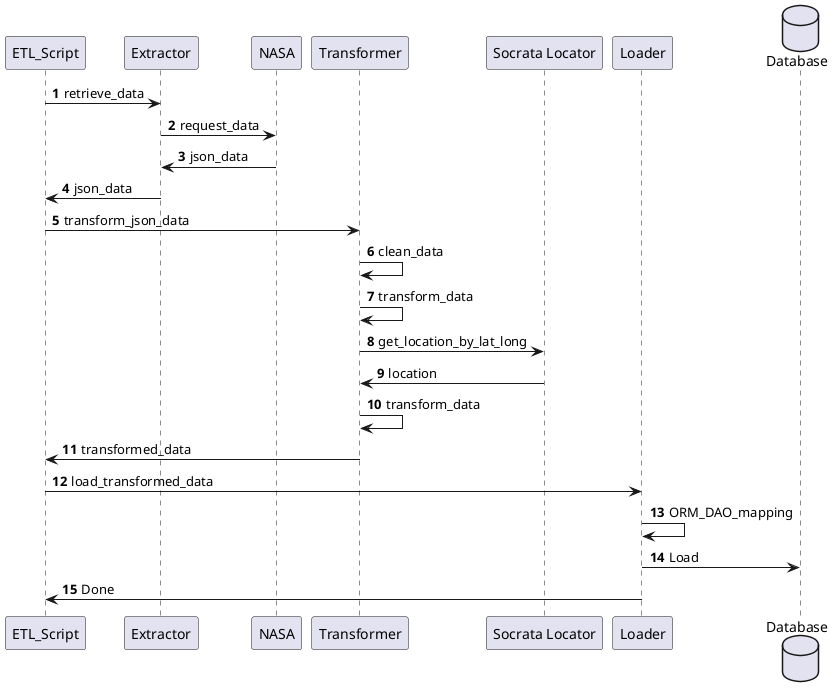
\includegraphics[width=\columnwidth]{images/sequence_diagram_etl.png}
		\caption{ETL Sequence Diagram}
		\label{fig:ETL Sequence Diagram}
	\end{figure}
	
	Details of these modules are described in the following sections.
	\subsection{Extract}
    Extraction is the process that allows us to obtain data from sources, and we know that this operation can be either static (generally used when the DWH needs to be populated for the first time) or incremental (used to update the DWH regularly). Since our datasets are not updated at regular intervals, we have decided to implement only static extraction. If an update is required, we will back up the previous DWH and then populate a new DWH system.\\ The extractor has 2 mainly problems to solve:
    \begin{itemize}
    	\item Navigate through the API pagination, to retrieve all data
    	\item Produce the raw object contained all data read by NASA
    \end{itemize}
    The Extractor class manages pagination by adjusting the offset parameter in its API requests. This ensures that all available data is retrieved by making multiple requests, each fetching a different segment of the data.
    The NASA dataset contains the information shown in the table \ref{tab:nasa_dataset}:
    \begin{table}[httb]
    	\centering
    	\caption{Meteorite Landings dataset}
    	\begin{tabular}{|p{1cm}|p{4cm}|p{1cm}|p{1cm}|}
    		\hline
    		\textbf{Name} & \textbf{Description} & \textbf{Field name} & \textbf{Datatype} \\ \hline
    		name & Meteorite Name & name & Text \\ \hline
    		id   & Meteorite Identifier  & id & Text \\ \hline
    		nametype & Relict meteorite or valid & nametype & Text \\ \hline
    		recclass & Meteorite Classification & recclass & Text \\ \hline
    		mass & Meteorite Mass (grams) & mass & Number \\ \hline
    		fall & Meteorite Fall on the earth or not & fall & Text \\ \hline
    		year & Event data (FLoating timestamp) & year & Floating timestamp \\ \hline
    		reclat & Latitude of the event & reclat & Text \\ \hline
    		reclong & Longitude of the event & reclong & Text \\ \hline
    	\end{tabular}
    	\label{tab:nasa_dataset}
    \end{table}
	For clarity, the API exposed by the \texttt{Extractor} class is shown in Figure \ref{fig:Extractor}. This figure provides a visual representation of the class's methods and their interactions with the NASA Meteorite Landings API.
	\begin{figure}[htpb]
		\centering
		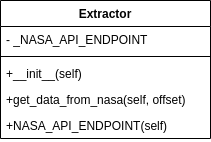
\includegraphics[width=0.5\columnwidth]{images/Extractor.png}
		\caption{Extractor Object}
		\label{fig:Extractor}
	\end{figure}

	\subsection{Transform}
	This process is computed by the \texttt{Transformer} class that provide a suite of methods to perform the transform process.\\ This class needs the raw data from the \texttt{Executor} to perform the following tasks:
	\begin{enumerate}
		\item Remove all meteorites containing not valid values
		\item Transform the filed \texttt{year} according with the dimension Date
		\item Transform the coordinate according with the dimension location
		\item Transform the classification according with the dimension classification
	\end{enumerate}
	
	\subsubsection{Remove all meteorites containing not valid values}
	This task is computed by the private function \texttt{clean}. This method returns a \texttt{MeteoriteLandingRaw} if the object can be transformed or a null value if the object is not valid. This function checks if the required fields are not null, empty and if the Geo Location coordinates can be suitable or not (are in the continents boundary and are not in a remote area).
	In figure \ref{fig:MeteoriteLandingRaw} is shown the \texttt{MeteoriteLandingRaw}
	\begin{figure}[htpb]
		\centering
		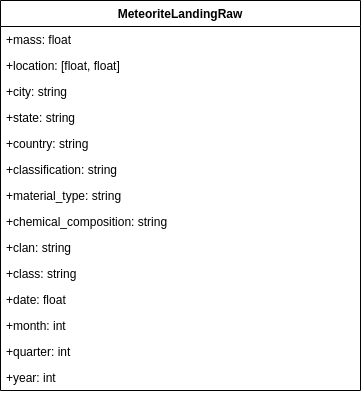
\includegraphics[width=\columnwidth]{images/meteorite_landing_raw.png}
		\caption{Meteorite Landing Raw Object}
		\label{fig:MeteoriteLandingRaw}
	\end{figure}
	
	
	\subsubsection{Date transformation}
	The transformation process continues on the field \texttt{year} that is a timestamp representation, then using the \texttt{DimensionDateModel} class we are able to perform this action computing year, month, quarter, timestamp. In Figure \ref{fig:DimensionDateModel} is shown the class diagram of this class:
	\begin{figure}[htpb]
		\centering
		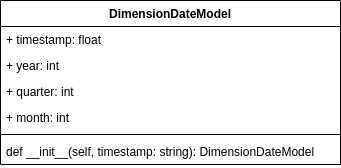
\includegraphics[width=\columnwidth]{images/dimension_date_model.png}
		\caption{Dimension Date Model Object}
		\label{fig:DimensionDateModel}
	\end{figure}
	
	At the end of the transform process is possible have in RAM the software structure compliant with the Class Diagram shown in Figure \ref{fig: ORM_mapping}.\\
	
	
	\subsubsection{Transform the coordinate according with the dimension location}
	This is task requires some technical limitation to be accomplished:
	\begin{itemize}
		\item Rate limit to use Reverse Geocoding APIs.
		\item Limited resources to install a local OpenStreetMap server or using a own database
		\item Free APIs don't allow multiple requests per second then is not possible to use threading algorithms to perform this task
	\end{itemize}
	
	This means that we need to optimize the algorithm to perform this transformation. Therefore we uses these criterias:
	\begin{itemize}
		\item Accuracy reduction of coordinates using one only decimal place, because in this manner we are able to recover the grandularity of our interest (State, Country and City), for more details see \href{https://en.wikipedia.org/wiki/Decimal_degrees#Precision}{Decimal Degrees Precision}
		\item Using a cache system on the RAM to store all processed coordinate and then call the remote API \texttt{iff} the value is not present in the cache
		\item Implemented an infinite Re-Try mechanism if a request fails, until it is not correctly processed
		\item Avoid multiple and burst requests to the remote API server (Avoid to be blacklisted) 
	\end{itemize}
	The image in the Figure \ref{fig:flow_diagram_tranform_location} shown the Flow Chart releated at this phese:
	\begin{figure}[htpb]
		\centering
		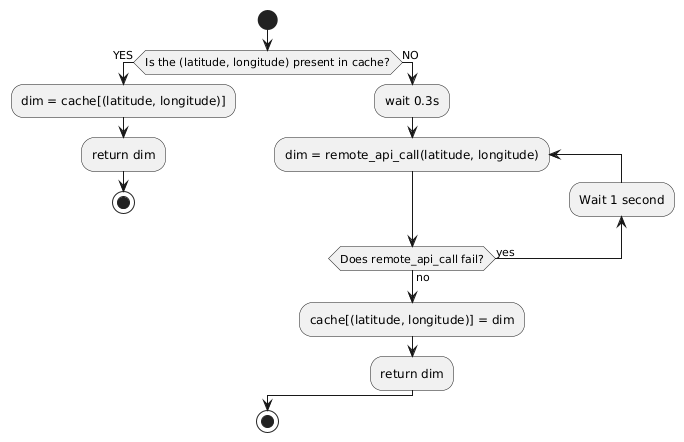
\includegraphics[width=\columnwidth]{images/flow_diagram_tranform_location.png}
		\caption{Transformation Location: Flow Chart}
		\label{fig:flow_diagram_tranform_location}
	\end{figure}
	
	With this algorithm the transformation process requires around one hour and half to reverse the geolocation of all data (46K geolocations).
	
	In the Figure \ref{fig:DimensionLocationModel} is shown the releated class:
	\begin{figure}[htpb]
		\centering
		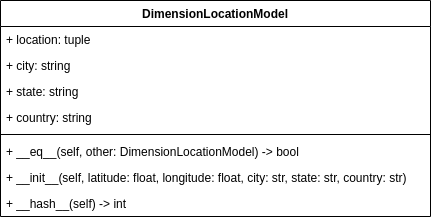
\includegraphics[width=\columnwidth]{images/dimension_location_model.png}
		\caption{Dimension Location Model Object}
		\label{fig:DimensionLocationModel}
	\end{figure}
	
	
	\subsubsection{Transform the classification according with the dimension classification}

	
	\subsection{Load}
	The Loader is the module responsible to load the data on the DWH, this is the reason why we decided that this module builds the mapping between the database and the software. In the Figure \ref{fig: ORM_mapping} is illustrated the mapping between the database tables and the software classes.\\ We used \texttt{SQLAlchemy} library to manage the DB schema.\\ This module is responsabile to:
	\begin{itemize}
		\item Enstablish a database connection with the DWH
		\item Mapping using the ORM approach the software layer with the database layer
		\item Insert atomically the data retrieved from the Transaltor to the right tables
	\end{itemize}
	
	\begin{figure}[htpb]
		\centering
		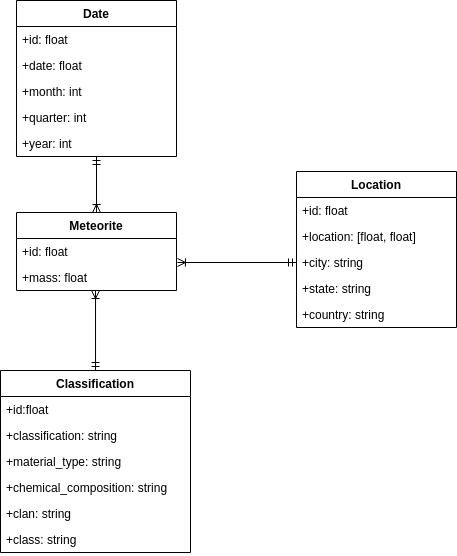
\includegraphics[width=\columnwidth]{images/uml_schema.png}
		\caption{ORM - UML Schema}
		\label{fig: ORM_mapping}
	\end{figure}
		
	\section{Conclusion}
	At the end of this work we have the DWH that can be queried through the SQL queries or other clients. For example it is possible to have a multidimensional view of data joining the fact table to its dimensions tables:\\
	\begin{verbatim}
		SELECT *
		FROM Meteorite AS FT, 
		Location AS DT1, 
		Date AS DT2, 
		Classification AS DT3
		WHERE 
		FT.Location = DT1.id AND 
		FT.Date = DT2.id AND
		FT.Classification = DT3.id
	\end{verbatim}
	
	
	\section{Source code}
	
	\section{Reference}
	\begin{itemize}
		\item \href{https://www.diag.uniroma1.it/~lenzerin/index.html/?q=node/53}{Data Management Course}
		\item \href{https://web.pdx.edu/~ruzickaa/meteorites/papers/WeisbergEtal2006-classification.pdf}{Weisberg et al. (2006) Systematics and Evaluation of Meteorite Classification. In, Meteorites and the Early Solar System II, 19-52 (D.S. Lauretta and H.Y. McSween, Eds.), Univ. Arizona press}
		\item \href{https://data.nasa.gov/Space-Science/Meteorite-Landings/gh4g-9sfh/about_data}{NASA's Open Data Portal}
		\item \href{https://photon.komoot.io/}{Photon - Open Street Map}
		\item \href{https://en.wikipedia.org/wiki/Decimal_degrees#Precision}{Decimal Degrees Precision}
	\end{itemize}
\end{document}
